\documentclass[aspectratio=169,10pt]{beamer}
\usetheme{Madrid}
\usecolortheme{default}
\setbeamertemplate{navigation symbols}{}

\usepackage[utf8]{inputenc}
\usepackage[T1]{fontenc}
\usepackage[brazil]{babel}
\usepackage{lmodern}
\usepackage{tikz}
\usetikzlibrary{shapes.geometric,positioning,calc,fit}
\usepackage{adjustbox}
\usepackage[normalem]{ulem}
\usepackage{booktabs}
\usepackage{tabularx}
\usepackage{array}

\newcolumntype{Y}{>{\raggedright\arraybackslash}X}
\newcolumntype{C}[1]{>{\centering\arraybackslash}p{#1}}

% =====================================================================
% Estilo dos diagramas ER/ERE -- notação Elmasri & Navathe,
% cores inspiradas na ferramenta TerraER
% (entidade verde, relacionamento amarelo, atributo lilás).
% Tamanhos de fonte podem ser redefinidos antes do \input.
% =====================================================================
\definecolor{terraEnt}{RGB}{186,242,186}
\definecolor{terraEntB}{RGB}{40,110,40}
\definecolor{terraRel}{RGB}{255,240,90}
\definecolor{terraRelB}{RGB}{120,100,0}
\definecolor{terraAtt}{RGB}{170,170,238}
\definecolor{terraAttB}{RGB}{40,40,120}

\providecommand{\erEntFont}{\scriptsize}
\providecommand{\erRelFont}{\tiny}
\providecommand{\erAttFont}{\tiny}
\providecommand{\erEntW}{2.3cm}
\providecommand{\erEntH}{0.7cm}
\providecommand{\erAttH}{0.42cm}

\tikzset{
  ent/.style={draw=terraEntB, semithick, rectangle, minimum width=\erEntW,
              minimum height=\erEntH, font=\sffamily\erEntFont, fill=terraEnt},
  went/.style={ent, double, double distance=1.5pt},
  rel/.style={draw=terraRelB, semithick, diamond, aspect=2.4, inner sep=1pt,
              font=\sffamily\erRelFont, fill=terraRel},
  irel/.style={rel, double, double distance=1.5pt},
  att/.style={draw=terraAttB, ellipse, inner sep=0.6pt, minimum height=\erAttH,
              font=\sffamily\erAttFont, fill=terraAtt},
  mval/.style={att, double, double distance=1pt},
  der/.style={att, dashed},
  spec/.style={draw, thick, circle, inner sep=0pt, minimum size=0.5cm,
               font=\sffamily\erEntFont, fill=white},
  tot/.style={double, double distance=1.6pt, line width=0.6pt},
  card/.style={midway, auto, inner sep=1.5pt, font=\sffamily\erEntFont},
  aggr/.style={draw=terraEntB, thick, rectangle, inner sep=0.35cm},
  sub/.style={midway, sloped, allow upside down, font=\small, inner sep=0pt},
}
\newcommand{\pk}[1]{\underline{#1}}
\newcommand{\ppk}[1]{\dashuline{#1}}

\newcommand{\diag}[1]{\begin{adjustbox}{max width=\linewidth, max totalheight=0.80\textheight, center}#1\end{adjustbox}}

% rodapé: só "TP1"
\setbeamertemplate{footline}{%
  \begin{beamercolorbox}[wd=\paperwidth,ht=2.5ex,dp=1ex,center]{title in head/foot}%
    \usebeamerfont{title in head/foot}TP1%
  \end{beamercolorbox}}

\usepackage{graphicx}

\title[TP I -- Modelagem Conceitual]{Sistema de Alocação de Quadras da UFOP}
\subtitle{Trabalho Prático I -- Modelagem Conceitual de Dados (ERE)}
\author[Pedro Souza et al.]{Pedro Souza \and Luiz Felipe Bento \and Gabriel Canuto \\ David Cristian \and Marcus Leandro \and Pedro Henrique Boseja}
\institute[UFOP]{BCC321 -- Banco de Dados I \\ Prof. Guilherme Tavares de Assis \\ DECOM / ICEB / UFOP}
\date{2026/2}

\begin{document}

\begin{frame}
  \titlepage
\end{frame}

% =====================================================================
\section{Minimundo}
% =====================================================================

\begin{frame}{Minimundo -- O sistema}
  \large
  \begin{itemize}
    \item Agendamento das quadras e campos da UFOP
    \item Evita conflitos de horário e reservas sem controle
    \item Alunos e organizações reservam; funcionários administram
  \end{itemize}
\end{frame}

\begin{frame}{Minimundo -- Quem usa}
  \large
  \begin{itemize}
    \item Usuário comum (aluno): reserva e participa
    \item Funcionário: abre os horários dos espaços, bloqueia, cancela e dá suporte
    \item Administrador: gerencia os funcionários
    \item Organização (atlética, DCE...): também pode reservar
  \end{itemize}
\end{frame}

\begin{frame}{Minimundo -- Como funciona}
  \large
  \begin{itemize}
    \item Cada espaço (quadra ou campo) fica em um campus
    \item O agendamento reserva um espaço + modalidade, em uma data,
          ocupando um ou mais blocos de 1 hora do horário aberto
    \item Pode ser cancelado, e o espaço pode ser bloqueado
    \item Usuários podem abrir chamados de suporte
  \end{itemize}
\end{frame}

% =====================================================================
\section{ERE}
% =====================================================================

\begin{frame}{ERE completo}
  \centering
  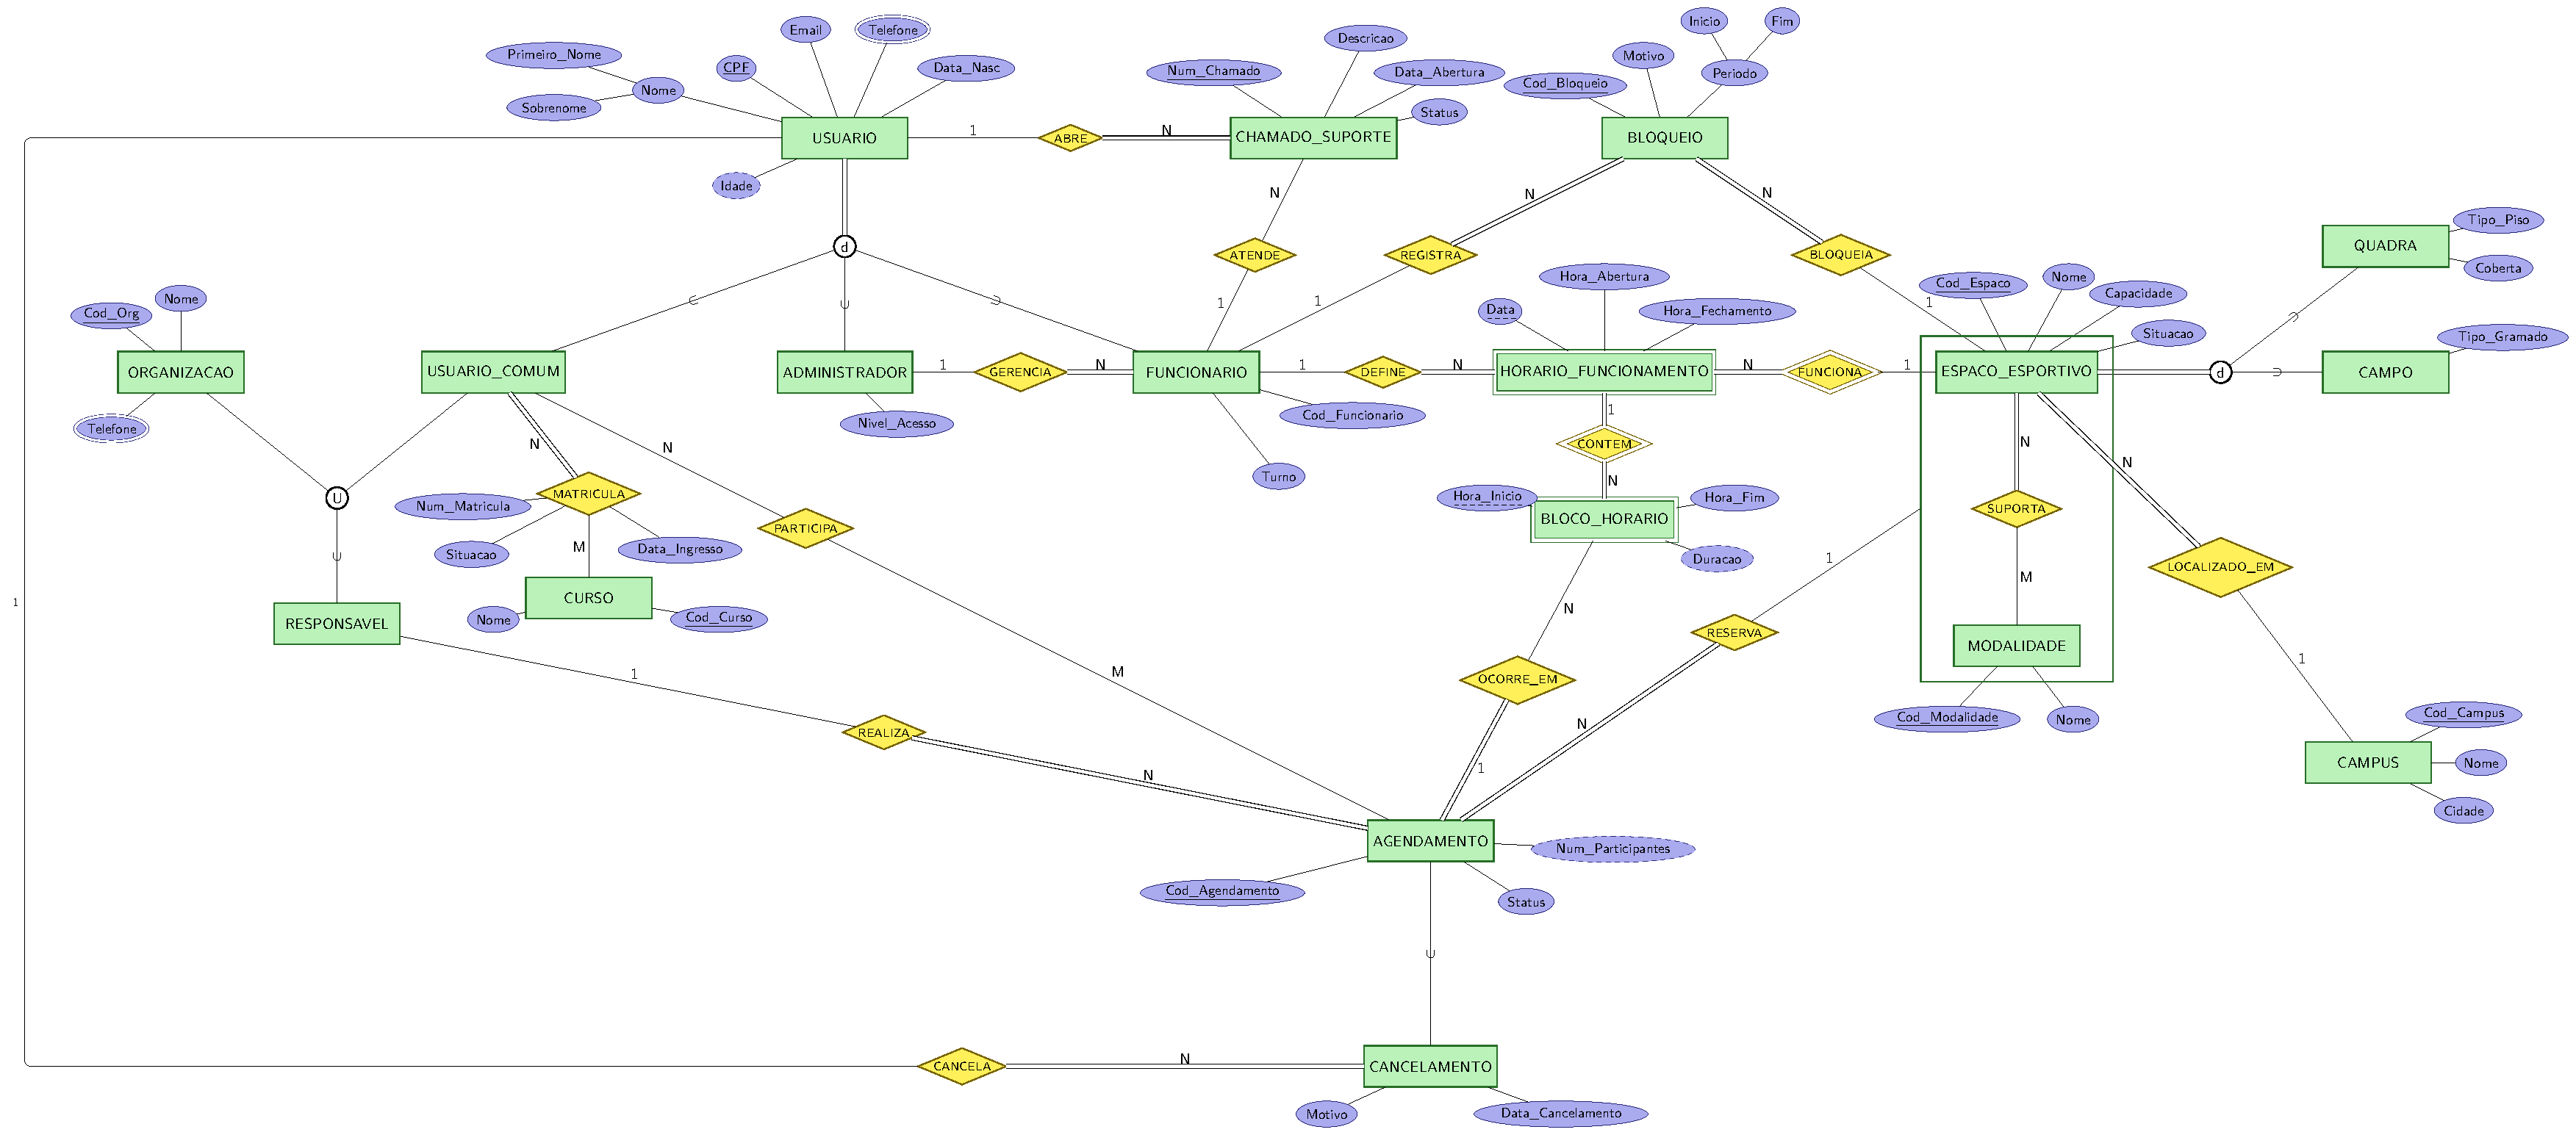
\includegraphics[width=\linewidth,height=0.86\textheight,keepaspectratio]{der.pdf}
\end{frame}

\begin{frame}{ERE -- detalhe (1/4): Usuários, curso, especialização e união}
\diag{\begin{tikzpicture}
  % USUARIO
  \node[ent] (U) at (0,3) {USUARIO};
  \node[att] (u1) at (-2.9,4.2) {\pk{CPF}};
  \node[att] (u2) at (-3.5,3) {Nome};
  \node[att] (u21) at (-5.7,3.6) {Primeiro\_Nome};
  \node[att] (u22) at (-5.7,2.4) {Sobrenome};
  \node[att] (u3) at (-1.0,4.7) {Email};
  \node[mval] (u4) at (1.0,4.7) {Telefone};
  \node[att] (u5) at (2.9,4.2) {Data\_Nasc};
  \node[der] (u6) at (3.5,3) {Idade};
  \foreach \a in {u1,u2,u3,u4,u5,u6} \draw (\a)--(U);
  \draw (u21)--(u2) (u22)--(u2);
  % especialização
  \node[spec] (d1) at (0,1.6) {d};
  \draw[tot] (U)--(d1);
  \node[ent] (UC) at (-5,0) {USUARIO\_COMUM};
  \node[ent] (F) at (0,0) {FUNCIONARIO};
  \node[ent] (A) at (5.5,0) {ADMINISTRADOR};
  \draw (d1)--node[sub]{$\supset$}(UC);
  \draw (d1)--node[sub]{$\supset$}(F);
  \draw (d1)--node[sub]{$\supset$}(A);
  % CURSO e MATRICULA (relacionamento M:N com atributos do par aluno/curso)
  \node[rel] (MR) at (-3.7,-1.6) {MATRICULA};
  \node[ent] (CU) at (-2.6,-3.3) {CURSO};
  \draw[tot] (UC)--node[card,swap]{N}(MR);
  \draw (MR)--node[card,swap]{M}(CU);
  \node[att] (mr1) at (-5.6,-2.6) {Num\_Matricula};
  \node[att] (mr2) at (-5.0,-3.5) {Data\_Ingresso};
  \node[att] (mr3) at (-1.0,-2.4) {Situacao};
  \foreach \a in {mr1,mr2,mr3} \draw (\a)--(MR);
  \node[att] (cu1) at (-3.6,-4.5) {\pk{Cod\_Curso}};
  \node[att] (cu2) at (-1.4,-4.4) {Nome};
  \foreach \a in {cu1,cu2} \draw (\a)--(CU);
  \node[att] (f1) at (-1.2,-1.3) {Cod\_Funcionario};
  \node[att] (f3) at (1.2,-1.3) {Turno};
  \draw (f1)--(F) (f3)--(F);
  \node[att] (a1) at (5.5,-1.3) {Nivel\_Acesso};
  \draw (a1)--(A);
  % GERENCIA
  \node[rel] (G) at (2.75,0) {GERENCIA};
  \draw (A)--node[card]{1}(G);
  \draw[tot] (G)--node[card]{N}(F);
  % ORGANIZACAO e união
  \node[ent] (O) at (-10,0) {ORGANIZACAO};
  \node[att] (o1) at (-11.6,1.2) {\pk{Cod\_Org}};
  \node[att] (o2) at (-10,1.5) {Nome};
  \node[mval] (o4) at (-11.9,-1.0) {Telefone};
  \foreach \a in {o1,o2,o4} \draw (\a)--(O);
  \node[spec] (un) at (-7.5,-2.4) {U};
  \draw (O)--(un) (UC)--(un);
  \node[ent] (R) at (-7.5,-3.9) {RESPONSAVEL};
  \draw (un)--node[sub]{$\supset$}(R);
\end{tikzpicture}
}
\end{frame}

\begin{frame}{ERE -- detalhe (2/4): Espaços, horário de funcionamento e agregação}
\diag{\begin{tikzpicture}
  \node[ent, minimum width=2.9cm] (E) at (0,3) {ESPACO\_ESPORTIVO};
  \node[att] (e2) at (-0.9,4.8) {\pk{Cod\_Espaco}};
  \node[att] (e3) at (0.8,4.9) {Nome};
  \node[att] (e4) at (2.4,4.5) {Capacidade};
  \node[att] (e5) at (3.3,3.8) {Situacao};
  \foreach \a in {e2,e3,e4,e5} \draw (\a)--(E);
  % especialização
  \node[spec] (d2) at (0,1.2) {d};
  \draw[tot] (E)--(d2);
  \node[ent] (Q) at (-2.6,-0.6) {QUADRA};
  \node[ent] (C) at (2.6,-0.6) {CAMPO};
  \draw (d2)--node[sub]{$\supset$}(Q);
  \draw (d2)--node[sub]{$\supset$}(C);
  \node[att] (q1) at (-3.5,-1.9) {Tipo\_Piso};
  \node[att] (q2) at (-1.8,-2.0) {Coberta};
  \draw (q1)--(Q) (q2)--(Q);
  \node[att] (k1) at (2.6,-1.9) {Tipo\_Gramado};
  \draw (k1)--(C);
  % MODALIDADE e agregação [ESPACO -- SUPORTA -- MODALIDADE]
  \node[rel] (S) at (-4.4,3) {SUPORTA};
  \node[ent] (M) at (-8.4,3) {MODALIDADE};
  \draw[tot] (E)--node[card,swap]{N}(S);
  \draw (S)--node[card,swap]{M}(M);
  \node[att] (m1) at (-9.4,1.6) {\pk{Cod\_Modalidade}};
  \node[att] (m2) at (-7.2,1.6) {Nome};
  \draw (m1)--(M) (m2)--(M);
  \node[aggr, fit=(M)(S)(E)] (AGR) {};
  % HORARIO_FUNCIONAMENTO (entidade fraca): espaço aberto em uma data
  \node[irel] (FU) at (4.6,1.4) {FUNCIONA};
  \node[went, minimum width=3.4cm] (HF) at (8.4,0.2) {HORARIO\_FUNCIONAMENTO};
  \draw (E)--node[card]{1}(FU);
  \draw[tot] (FU)--node[card]{N}(HF);
  \node[att] (hf1) at (6.9,-1.1) {\ppk{Data}};
  \node[att] (hf2) at (8.5,-1.4) {Hora\_Abertura};
  \node[att] (hf3) at (10.3,-1.0) {Hora\_Fechamento};
  \foreach \a in {hf1,hf2,hf3} \draw (\a)--(HF);
  % CAMPUS
  \node[rel] (L) at (5.4,3) {LOCALIZADO\_EM};
  \node[ent] (CA) at (9.2,3) {CAMPUS};
  \draw[tot] (E)--node[card]{N}(L);
  \draw (L)--node[card]{1}(CA);
  \node[att] (ca1) at (7.9,4.2) {\pk{Cod\_Campus}};
  \node[att] (ca2) at (9.5,4.5) {Nome};
  \node[att] (ca3) at (10.8,4.0) {Cidade};
  \foreach \a in {ca1,ca2,ca3} \draw (\a)--(CA);
\end{tikzpicture}
}
\end{frame}

\begin{frame}{ERE -- detalhe (3/4): Agendamento, blocos de horário e cancelamento}
\diag{\begin{tikzpicture}
  \node[ent, minimum width=2.6cm] (AG) at (0,0) {AGENDAMENTO};
  \node[att] (g1) at (-1.6,1.5) {\pk{Cod\_Agendamento}};
  \node[att] (g3) at (1.9,1.5) {Status};
  \node[der] (g4) at (2.9,0.8) {Num\_Participantes};
  \foreach \a in {g1,g3,g4} \draw (\a)--(AG);
  % REALIZA
  \node[rel] (RE) at (-4.6,0) {REALIZA};
  \node[ent] (R) at (-8.4,0) {RESPONSAVEL};
  \draw (R)--node[card]{1}(RE);
  \draw[tot] (RE)--node[card]{N}(AG);
  % PARTICIPA
  \node[rel] (PA) at (-4.6,-1.9) {PARTICIPA};
  \node[ent, minimum width=2.7cm] (UC) at (-8.4,-1.9) {USUARIO\_COMUM};
  \draw (UC)--node[card]{N}(PA);
  \draw (PA)--node[card]{M}(AG);
  % RESERVA -> agregação [ESPACO -- SUPORTA -- MODALIDADE]
  \node[ent, minimum width=2.9cm] (E) at (9.4,1.6) {ESPACO\_ESPORTIVO};
  \node[rel] (SU) at (9.4,0) {SUPORTA};
  \node[ent] (M) at (9.4,-1.6) {MODALIDADE};
  \draw[tot] (E)--node[card]{N}(SU);
  \draw (SU)--node[card]{M}(M);
  \node[aggr, fit=(E)(SU)(M)] (AGR) {};
  \node[rel] (RS) at (4.9,0) {RESERVA};
  \draw[tot] (AG)--node[card]{N}(RS);
  \draw (RS)--node[card]{1}(AGR.west);
  % OCORRE_EM -> BLOCO_HORARIO (um agendamento ocupa um ou mais blocos)
  \node[rel] (OE) at (4.0,-2.6) {OCORRE\_EM};
  \node[went, minimum width=2.9cm] (H) at (8.0,-3.9) {BLOCO\_HORARIO};
  \draw[tot] (AG)--node[card,swap]{1}(OE);
  \draw (OE)--node[card,swap]{N}(H);
  \node[att] (h2) at (6.9,-5.2) {\ppk{Hora\_Inicio}};
  \node[att] (h3) at (8.9,-5.4) {Hora\_Fim};
  \node[der] (h4) at (10.4,-4.9) {Duracao};
  \foreach \a in {h2,h3,h4} \draw (\a)--(H);
  % CANCELAMENTO: subclasse de AGENDAMENTO (especialização parcial)
  \node[ent, minimum width=2.6cm] (CN) at (0,-3.9) {CANCELAMENTO};
  \draw (AG)--node[sub]{$\supset$}(CN);
  \node[att] (cn1) at (1.9,-5.1) {Data\_Cancelamento};
  \node[att] (cn2) at (-1.6,-5.1) {Motivo};
  \draw (cn1)--(CN) (cn2)--(CN);
  \node[rel] (CL) at (-4.6,-3.9) {CANCELA};
  \node[ent] (U) at (-8.4,-3.9) {USUARIO};
  \draw (U)--node[card]{1}(CL);
  \draw[tot] (CL)--node[card]{N}(CN);
  % blocos pertencem ao horário de funcionamento (entidade fraca)
  \node[irel] (CT) at (12.2,-3.9) {CONTEM};
  \node[went, minimum width=3.4cm] (HF) at (16.2,-3.9) {HORARIO\_FUNCIONAMENTO};
  \draw[tot] (HF)--node[card,swap]{1}(CT);
  \draw[tot] (CT)--node[card,swap]{N}(H);
\end{tikzpicture}
}
\end{frame}

\begin{frame}{ERE -- detalhe (4/4): Gestão: bloqueios, horários e suporte}
\diag{\begin{tikzpicture}
  \node[ent] (F) at (0,0) {FUNCIONARIO};
  % BLOQUEIO
  \node[rel] (RG) at (0,1.9) {REGISTRA};
  \node[ent] (B) at (0,3.8) {BLOQUEIO};
  \draw (F)--node[card]{1}(RG);
  \draw[tot] (RG)--node[card]{N}(B);
  \node[att] (b1) at (-2.4,4.4) {\pk{Cod\_Bloqueio}};
  \node[att] (b2) at (-1.0,5.1) {Motivo};
  \node[att] (b3) at (1.0,5.1) {Periodo};
  \node[att] (b31) at (0.3,6.1) {Inicio};
  \node[att] (b32) at (1.8,6.1) {Fim};
  \draw (b1)--(B) (b2)--(B) (b3)--(B) (b31)--(b3) (b32)--(b3);
  \node[rel] (BL) at (3.8,3.8) {BLOQUEIA};
  \node[ent, minimum width=2.9cm] (E) at (7.8,3.8) {ESPACO\_ESPORTIVO};
  \draw[tot] (B)--node[card]{N}(BL);
  \draw (BL)--node[card]{1}(E);
  % HORARIO_FUNCIONAMENTO (o funcionário abre o espaço em uma data)
  \node[rel] (DF) at (3.6,0) {DEFINE};
  \node[went, minimum width=3.4cm] (H) at (7.8,0) {HORARIO\_FUNCIONAMENTO};
  \draw (F)--node[card]{1}(DF);
  \draw[tot] (DF)--node[card]{N}(H);
  \node[irel] (FU) at (7.8,1.9) {FUNCIONA};
  \draw (E)--node[card]{1}(FU);
  \draw[tot] (FU)--node[card]{N}(H);
  % CHAMADO
  \node[rel] (AT) at (-3.8,0) {ATENDE};
  \node[ent] (CH) at (-7.6,0) {CHAMADO\_SUPORTE};
  \draw (F)--node[card]{1}(AT);
  \draw (AT)--node[card]{N}(CH);
  \node[att] (ch1) at (-10.1,0.9) {\pk{Num\_Chamado}};
  \node[att] (ch3) at (-7.8,1.6) {Descricao};
  \node[att] (ch4) at (-6.2,1.4) {Data\_Abertura};
  \node[att] (ch5) at (-5.5,0.8) {Status};
  \foreach \a in {ch1,ch3,ch4,ch5} \draw (\a)--(CH);
  \node[rel] (AB) at (-7.6,-1.6) {ABRE};
  \node[ent] (U) at (-7.6,-3.0) {USUARIO};
  \draw (U)--node[card]{1}(AB);
  \draw[tot] (AB)--node[card]{N}(CH);
\end{tikzpicture}
}
\end{frame}

\begin{frame}
  \centering\Huge Obrigado!\par\vspace{0.5em}
  \large Dúvidas?
\end{frame}

\end{document}
